\chapter{Patient journey}
This chapter defines the patient journey, collection of historical data of patients from the beginning of treatment. After performing information loss analytics to validate the approach, couples of diagnoses-prescriptions are identified to observe their relationship.

After a preliminary analysis to underline the main focus areas, there is enough information to begin reconstructing the \textbf{patient journey}, a complete set of data including a patient's records and relationships with primary healthcare, to then identify patterns and changes. 

An objective definition of patient journey can be created using the following guidelines:
\begin{enumerate}
	\item Patients with \textbf{complete medical history} for a fixed amount of years;
	\item Records with patient, prescribing GP, diagnosis and prescription on the \textbf{same date};
	\item Only \textbf{first-time} diagnoses and prescriptions considered.
\end{enumerate}

The imposed criteria is strict: taking diagnoses and prescriptions on the same day means removing \textit{all prescriptions} following the first diagnosis. In other words, all the instances of patients coming back to their GP to renew a prescription (e.\ g. for a chronic disease) have been deleted.

This approach can be useful to extract a cohort of patients beginning their treatment, and analyse the variations of first-time prescriptions, especially for chronic illnesses. It's important to notice that \textbf{not all doctors} may have patients getting new diagnoses.

\section{Imposed criteria}
Aside from completeness and correctness of the data, there are more restrictions to maintain consistency:
\begin{itemize}
	\item The prescribing general practitioner should not change in the time range;
	\item The patient should not be deceased;
	\item There should be a sanitary convention;
	\item The general practitioner should be active.
\end{itemize}

All those constraints can be checked using the related fields in the database: \textit{revocation} for interruption of the relationship, \textit{death} for death and \textit{convention} for the sanitary convention.

The table \textit{users} contains all the IDs of active general practitioners in 2018, therefore joining it with other tables is the best method to remove all the rows with an inactive GP. Data is up to date, and since the patient journey includes 2018 and requires consistency of history (the focus is on the most recent information) there is no need to check for active GPs in the previous years.

The biggest risk is again the \textbf{loss of information}: the impact of data cleansing is heavy, and the obtained results might not give an insightful perspective.

\section{Examples of data cleaning}
An initial data cleaning has been made on the whole database to have a first understanding of the potential information loss.

In this case, having such a big amount of tuples is useful: it is possible to remove a considerable percentage of them without losing generality and still having numerous samples.

Information on the general loss is already available thanks to the specific analysis on each single field, therefore the shown data cleaning will only consider patients and GPs.

The active general practitioners are \textbf{432}: this result has been retrieved counting the different IDs in \textit{users} (438) and removing the ones not present in \textit{patients\_doctors} (6).

About half of patients is going to be lost, due to not respecting the consistency criteria. Starting from a million of records, concrete results are still obtainable.

\subsection{ICD-9}
ICD-9 codes have been removed after a comparison with the official WHO database.

The 2 669 312 removed tuples have the following issues:
\begin{itemize}
	\item Wrong code: 0.005\%;
	\item Empty code: 75.4\%;
	\item Empty description: 24.6 \%.
\end{itemize}

The total number of rows is 15 460 199, of which 17\% must be deleted due to falling among one of the above categories.

\subsection{ATC}
ATC have been removed according to the same procedure as ICD-9.

The 3 328 041 removed tuples have the following issues:
\begin{itemize}
	\item Wrong code: 52.6\%;
	\item Empty code: 47.4\%.
\end{itemize}

Those consist in 21,5\% of total.

Further statistics related to data loss are extracted after having a first set of results, comparing individual values to the original after each step of restriction imposition. 

\section{Patient-based approach}
The first approach consists in testing with an \textbf{arbitrary range constraint}: all dates must fall in the span between 2010 and 2018.

The first analysis has pure research and testing purposes, to understand the impact of cutting the dataset in terms of information loss. All the previously introduced criteria must be considered as well: there must be a continuous doctor-patient relationship between active GPs and non-deceased patients with sanitary conventions.

To summarise, the obtained slice of data comprehends only patients starting their journey from 2010, having diagnosis and prescription on the same date by an active GP.

The outcome is a patient journey table containing data from 2000 to 2018, with a total amount of \textbf{144 618} tuples: this means that there are roughly 150k first-time diagnoses and prescriptions to patients. 

\subsection{Results breakdown}
Seeing that the starting tables had number of rows in the order of millions, some deeper analysis is necessary to figure out the uses of this significant loss.

The 144 618 complete tuples are composed by:
\begin{itemize}
	\item 27 733 patients;
	\item 422 general practitioners;
	\item 1 381 unique diagnoses;
	\item 904 unique prescriptions.
\end{itemize}

Further uses for those low values can be found counting how many dates would not fall in the considered range. The percentage of records with date earlier than 2010 in each table is:
\begin{itemize}
	\item Patients: 75\%;
	\item Diagnoses: 54.6\%;
	\item Prescriptions: 44.7\%.
\end{itemize}

It can be seen that most data loss is used by patients, most likely starting their treatment prior to 2010.

\subsubsection{Patients}
The following \textit{pie chart} illustrates the data loss on patients according to the criteria defined in the previous section.
\begin{figure}[h]
	\centering
	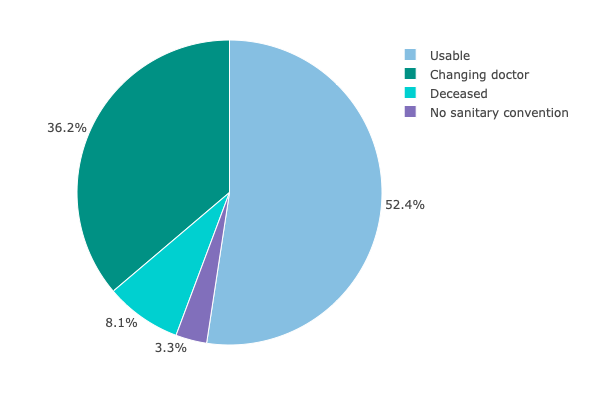
\includegraphics[scale=0.6]{images/patients-pie-1.png}
	\label{patientspie}
	\caption{\small Information loss on patients}
\end{figure}

The total amount of unusable patients is 58 415, not enough to use a loss of 75\%: the reason is therefore cutting off all data before 2010.

8 years is a too wide range to obtain a consistent patient journey, and such information loss isn't negligible: the conclusion of the first approach is that introducing time boundaries is something which needs an accurate control, to avoid missing out most of the data.

\section{Prescription-based approach}
Since extracting a slice of records according to their date span is an abrupt approach, careful parameter tuning and detailed constraints introduction is necessary to have a solid and consistent amount of information.

The focus is on the \textbf{number of prescriptions}: given a small range of years, only patients with \textit{at least one new prescription} are going to be considered. All the previous criteria must be respected (continuous doctor-patient relationship between active GPs and non-deceased patients with sanitary conventions).

This methodology allows cluster sampling without having to remove half of the dates: criteria based on the number of prescriptions creates another patient cohort which can be used to accurately select rows from the other tables.

The proposed time range is \textbf{2016-2018}: pharmaceutical companies generally use the last two years of sales, so picking the last three years gives additional information without compromising the consistency of data.

The outcome is a patient journey consisting of 1 465 005 tuples: almost 10 times the previous result. This leads to two important statements:
\begin{enumerate}
	\item The time range is appropriate, since the number is large enough to make analysis without loss of generality;
	\item The new imposed criterion gives more consistent data and the possibility to build time series.
\end{enumerate}

Further cleaning is required to link diagnoses and prescriptions, since there is not an univocal correspondence: multiple diagnosis and prescriptions may be associated to the same date. 

\subsection{Results breakdown}
The 1 465 005 complete tuples are composed by:
\begin{itemize}
	\item 230 381 patients;
	\item 412 general practitioners;
	\item 4 324 unique diagnoses;
	\item 1 280 unique prescriptions.
\end{itemize}

Only 7\% of the total prescriptions have been taken into account, yet a million and half is still a consistent amount.

\subsubsection{Funnel graph of patients}
A funnel chart is used to visualize the progressive reduction of data as it passes from one phase to another. Data in each of these phases is represented as different portions of 100\% (the whole amount of patients)\footnote{\href{https://www.fusioncharts.com/resources/chart-primers/funnel-chart}{Funnel chart, Fusioncharts}}.

\begin{figure}[h]
	\centering
	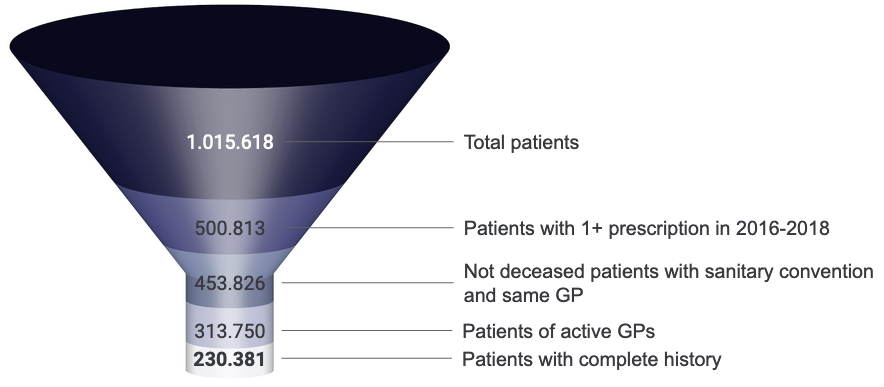
\includegraphics[scale=0.4]{images/funnel.png}
	\caption{\small Information loss on patients, funnel graph}
\end{figure}

Imposing every restriction made the patients number decrease: starting from a million, the remaining ones are $\nicefrac{1}{4}$ of it.

The constraint removing the biggest part consists in having at least one prescription, meaning that half of patients is generally healthy and most prescriptions are related to a smaller subset of individuals.

\subsection{Examples of analysis}
Resulting information, despite needing further checking and lookup, is a starting point for time series analysis.

\subsubsection{Prescription indicators}
There are 1 465 005 prescriptions, 1 280 of which are unique.

Average new prescriptions per patient:
\begin{table}[h]
	\centering
	\begin{tabular}{c|c}
		\textbf{Year} & \textbf{Average} \\
		\hline
		2016 & 3.26 \\
		\hline
		2017 & 3.37 \\
		\hline
		2018 (incomplete) & 3.06 \\
		\hline
		All years & 5.16
	\end{tabular}
	\caption{\small Average new prescriptions}
\end{table}

The range goes from 1 to 129 new prescriptions associated with diagnosis in three years.

\subsubsection{Most common couples}
The 5 most common diagnoses and prescriptions happening on the same day are displayed in the table below.
\begin{table}[h]
	\centering
	\begin{tabular}{c|c|c}
		\textbf{Diagnosis} & \textbf{Prescription} & \textbf{Count} \\
		\hline
		Vitamin D deficiency, unspecified & Colecalciferol & 13 122 \\
		\hline
		Periapical abscess without sinus & Amoxicillin and beta-lactamase inhibitor & 7 761 \\
		\hline
		Esophageal reflux & Pantoprazole & 6 093 \\
		\hline
		Diarrhea, unspecified & Rifaximin & 6 000 \\
		\hline
		Cystitis, unspecified & Fosfomycin & 5 885 \\
	\end{tabular}
	\caption{\small Most common couples of diagnosis-prescription}
\end{table}

The first one is a type of vitamin D, and Pantopranzole is a medicine for digestive tract diseases: all the others are antibiotics. 

This prior analysis already shows a concerning amount of antibiotic prescriptions. 

\subsubsection{Most common antibiotics}
Antibiotic prescriptions compose 20\% of total, which consists in 300 503 instances. The most popular ones are:
\begin{enumerate}
	\item Amoxicillin and beta-lactose inhibitors, 62 560 prescriptions;
	\item Ciprofloxacin, 23 762 prescriptions;
	\item Levofloxacin, 22 595 prescriptions;
	\item Rifaximin, 21 680 prescriptions;
	\item Ceftriaxone, 19 523 prescriptions.
\end{enumerate}

\section{Results comparison}
Comparing the two patient journey outcomes through graphs is a good way to visualize changes and improvements.

\subsection{Changes in data composition}
Figure \ref{barplots} shows barplots highlighting the changes between data categories in the two approaches.
\begin{figure}[h]
	\centering
	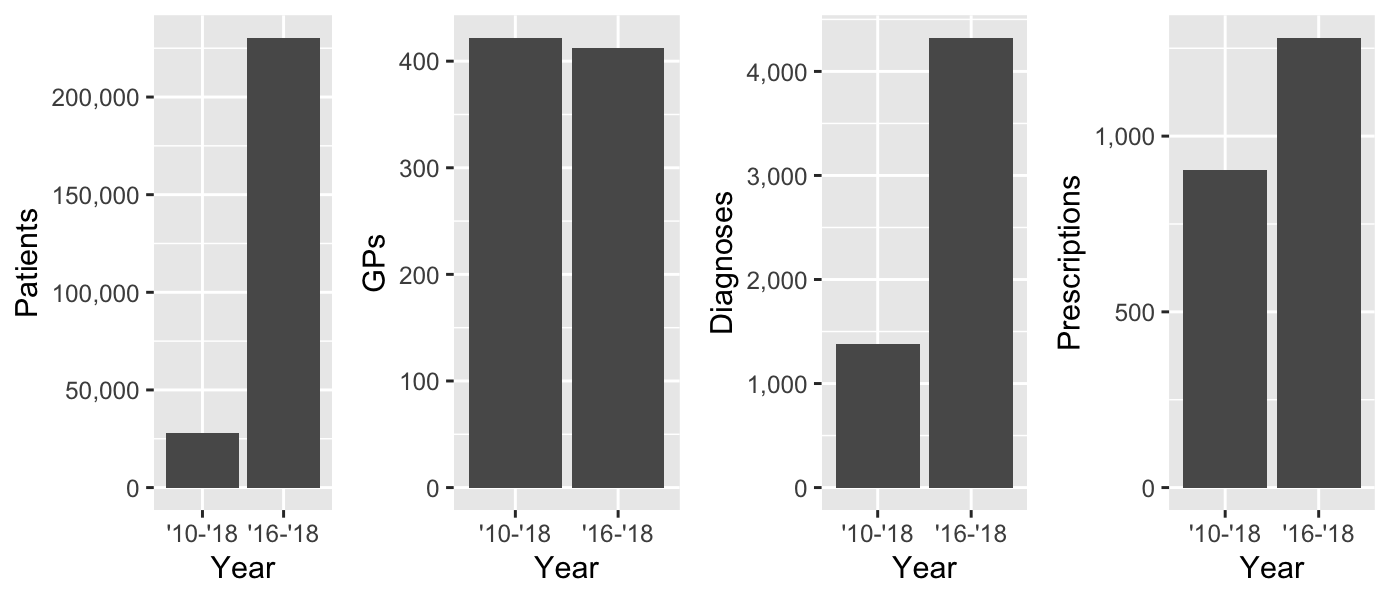
\includegraphics[scale=0.33]{../plots/pj-barplots.png}
	\caption{\small Information loss barplots}
	\label{barplots}
\end{figure}

General practitioners' number is stable, yet all the other categories are subject to a substantial improvement in the prescription-based approach.

Patients, in particular, change from 27 733 to 230 301.

\subsection{Improvement on patients information loss}
A pie chart for data loss on patients in the range 2016-2018 has been made to compare with the previous one.

\begin{figure}[h]
	\centering
	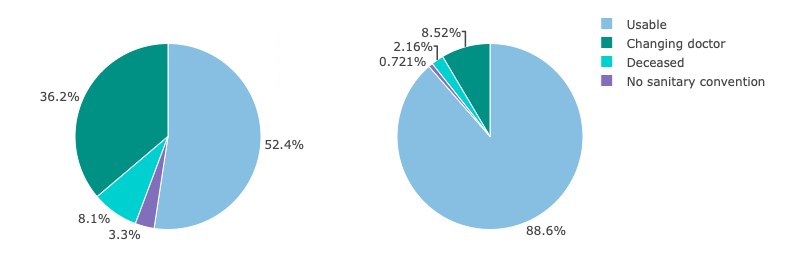
\includegraphics[scale=0.6]{images/patients-pies.png}
	\caption{\small Information loss comparison pie charts, 2010-2018 on left, 2016-2018 on right}
\end{figure}

It is confirmed that the number of usable patients has noticeably increased: using a smaller time span reduces the chances of death and change of GP.

\section{Future work}
Further analysis is needed to assess an insightful perspective focussed on specific diseases, including \textit{prescriptions following the first related diagnoses} and removing unrelated ones having the same date.

Examples of future work are:
\begin{itemize}
	\item Definition of a criterion so that a patient is considered chronic (minimum amount of prescriptions);
	\item Selection of GPs and patients having a number of diagnoses and prescription within a range (for data consistency);
	\item Deeper analysis of prescription changes during the years;
	\item Analysis on specific diseases (digestive system and tumours);
	\item Time series analysis and clustering approaches.
\end{itemize}

Since research shows a considerable amount of antibiotic instances, the data is linking to the issue of antibiotic resistance. More detailed analysis using time series can give a wider perspective.